\documentclass[pra,12pt]{revtex4}
\usepackage{amsmath}
\usepackage{amssymb}
\usepackage{graphicx}
\usepackage{color}
\usepackage{mathrsfs}
\usepackage{enumerate}
\usepackage{epigraph}
\usepackage[pdfborder={0 0 0},colorlinks=true,linkcolor=blue,urlcolor=blue]{hyperref}

\def\ket#1{\left|#1\right\rangle}
\def\bra#1{\left\langle#1\right|}
\def\braket#1{\left\langle#1\right\rangle}

\setlength{\parindent}{0pt}

\renewcommand{\baselinestretch}{1.0}
\setlength{\parskip}{0.07in}
\setlength{\epigraphwidth}{.6\textwidth}

\begin{document}

\begin{center}
{\Large \textbf{Chapter 4: Quantum Electrodynamics}}
\end{center}

This chapter describes \textbf{quantum electrodynamics}, the quantum
theory of the electromagnetic field and how it interacts with charged
particles such as electrons.  We start by formulating Hamiltonians
that describe how a quantum mechanical electron is affected by
classical electric and magnetic fields.  Next, we describe the
quantization of Maxwell's equations, which yields a quantum field
theory in which the elementary excitations are photons---particles of
light.  Finally, we can formulate a theory in which both electrons and
photons are treated on the same footing, as excitations of underlying
quantum fields.  Along the way, we will see how relativity is
accomodated into the framework of quantum mechanics.

Quantum electrodynamics is a rich and intricate theory, and we will
not be able to cover many important topics, such as diagrammatic
methods for performing field theoretical calculations.  If you are
interested in this topic, a good introductory textbook is Zee's
\textit{Quantum Field Theory in a Nutshell} (\hyperref[cite:zee]{Zee
  2010}).

\section{Particles in a classical electromagnetic field}

\subsection{Non-relativistic spinless particles}

Consider a non-relativistic charged particle in an electromagnetic
field.  As we are mainly interested in the physics of electrons
interacting with electromagnetic fields, we will henceforth take the
electric charge of the particle to be $-e$, where $e =
1.602\times10^{-19}\,\mathrm{C}$ is the elementary charge.  (If you
wish to describe particles with an arbitrary electric charge $q$,
simply perform the substitution $e \rightarrow -q$ in all formulas in
the rest of this chapter.)  For simplicity, we also assume (for now)
that the particle has charge and mass but is otherwise
``featureless''; in particular, unlike a real electron, it has no spin
angular momentum, and no magnetic dipole moment.

Suppose we treat the electromagnetic field as a classical field, in
the sense that the electric and magnetic field strengths are definite
quantities, not subject to quantum dynamics.  Our goal is to formulate
the Hamiltonian governing the quantum dynamics of this
non-relativistic charged particle.  To do this, let us first derive
the particle's \textit{classical} equations of motion.

In the classical regime, the action of an electromagnetic field on a
point charged particle is decribed by the Lorentz force law,
\begin{equation}
  \mathbf{F}(\mathrm{r},t) = -e\Big(\mathbf{E}(\mathrm{r},t)
  + \dot{\mathbf{r}}\times \mathbf{B}(\mathrm{r},t)\Big),
\end{equation}
where $\mathbf{r}$ and $\dot{\mathbf{r}}$ respectively denote the
position and velocity of the particle, $t$ is the time, and
$\mathbf{E}$ and $\mathbf{B}$ are the electric and magnetic fields.
If there are no other forces acting on the particle, then according to
Newton's second law, the equation of motion is
\begin{equation}
  m\ddot{\mathbf{r}} = -e\Big(\mathbf{E}(\mathrm{r},t)
  + \dot{\mathbf{r}} \times \mathbf{B}(\mathrm{r},t)\Big),
  \label{eom}
\end{equation}
where $m$ is the particle's mass.  To quantize this, we must convert
this equation of motion into the form of Hamilton's equations of
motion.

First, we introduce the electromagnetic scalar and vector potentials
$\Phi(\mathrm{r},t)$ and $\mathbf{A}(\mathrm{r},t)$, where
\begin{align}
  \mathbf{E}(\mathbf{r},t) &= - \nabla \Phi(\mathbf{r},t) - \frac{\partial\mathbf{A}}{\partial t} \\
  \mathbf{B}(\mathbf{r},t) &= \nabla \times \mathbf{A}(\mathbf{r},t).
  \label{Bfield}
\end{align}
We now postulate that the above equation of motion can be described by
the Lagrangian
\begin{equation}
  L(\mathbf{r},\dot{\mathbf{r}},t) = \frac{1}{2}m\dot{\mathbf{r}}^2
  + e \Big[\Phi(\mathbf{r},t) - \dot{\mathbf{r}} \cdot \mathbf{A}(\mathbf{r},t)
    \Big].
\end{equation}
This is very similar to the usual prescription for the Lagrangian as
the kinetic energy minus the potential energy, with $-e\Phi$ serving
as the potential energy function.  However, there is an extra
$-e\dot{\mathbf{r}} \cdot \mathbf{A}$ term; this will turn out to be
responsible for the magnetic force.  Let us plug the Lagrangian into
the Euler-Lagrange equations:
\begin{equation}
  \frac{\partial L}{\partial r_i} = \frac{d}{dt}
  \frac{\partial L}{\partial \dot{r}_i}.
\end{equation}
The partial derivatives of the Lagrangian are:
\begin{align}
  \begin{aligned}
    \frac{\partial L}{\partial r_i} &=
    e\Big[\partial_i \Phi - \dot{r}_j \,\partial_i A_j \Big]\\
    \frac{\partial L}{\partial \dot{r}_i} &= m\dot{r}_i - e A_i.
  \end{aligned}
\end{align}
Next, we want to take the \textit{total} time derivative of $\partial
L /\partial \dot{r}_i$.  In doing so, we note that the $\mathbf{A}$
field has its own $t$-dependence, as well as varying with the
particle's $t$-dependent position:
\begin{align}
  \begin{aligned}
    \frac{d}{dt} \frac{\partial L}{\partial \dot{r}_i}
    &= m\ddot{r}_i - e\, \frac{d}{dt} A_i(\mathbf{r}(t),t) \\
    &= m\ddot{r}_i - e\, \partial_t A_i
    - e\, \dot{r}_j \partial_j A_i.
  \end{aligned}
\end{align}
(In the above equations, $\partial_i \equiv \partial/\partial r_i$,
where $r_i$ is the $i$-th component of the position vector, while
$\partial_t \equiv \partial/\partial t$.)  Putting these results into
the Euler-Lagrange equations yields
\begin{align}
  \begin{aligned}
    m\ddot{r}_i &=
    -e\Big[\Big(-\partial_i \Phi - \partial_t A_i\Big)
      + \dot{r}_j \Big( \partial_i A_j - \partial_j A_i\Big) \Big] \\
    &= -e \Big[E_i(\mathbf{r},t) + \big(\dot{\mathbf{r}} \times
      \mathbf{B}(\mathbf{r},t) \big)_i\; \Big].
  \end{aligned}
\end{align}
(The last step can be derived by expressing the cross product using
the Levi-Cevita symbol, and using the identity $\varepsilon_{ijk}
\varepsilon_{lmk} = \delta_{il} \delta_{jm} - \delta_{im}
\delta_{jl}$.)  And indeed, this is the equation of motion
corresponding to the Lorentz force.

We can now derive the classical Hamiltonian.  First, we define the
canonical momentum:
\begin{equation}
  p_i = \frac{\partial L}{\partial \dot{r}_i} = m\dot{r}_i - e A_i.
\end{equation}
Now the Hamiltonian can be defined as $H(\mathbf{r},\mathbf{p}) =
\mathbf{p} \cdot \dot{\mathbf{r}} - L$, which needs to be expressed
using the $\mathbf{p}$ variables rather than $\dot{\mathbf{r}}$
variables:
\begin{align}
  \begin{aligned}
    H &= \mathbf{p}\cdot \left(\frac{\mathbf{p}+e\mathbf{A}}{m}\right)
    - \left(\frac{|\mathbf{p}+e\mathbf{A}|^2}{2m}
    + e\Phi - \frac{e}{m}(\mathbf{p}+e\mathbf{A})\cdot \mathbf{A}\right) \\
    &= \frac{|\mathbf{p}+e\mathbf{A}|^2}{m}
    - \frac{e}{m}\mathbf{A}\cdot \left(\mathbf{p}+e\mathbf{A}\right)
    - \left(\frac{|\mathbf{p}+e\mathbf{A}|^2}{2m}
    + e\Phi - \frac{e}{m}(\mathbf{p}+e\mathbf{A})\cdot \mathbf{A}\right)
  \end{aligned}
\end{align}
After cancelling various terms, we arrive at the result
$$\boxed{\qquad H = \frac{|\mathbf{p}+e\mathbf{A}(\mathbf{r},t)|^2}{2m} - e\Phi(\mathbf{r},t).\qquad}$$

This looks much like the familiar Hamiltonian for a non-relativistic
particle that we have dealt with many times,
\begin{equation}
  H = \frac{|\mathbf{p}|^2}{2m} + V(\mathbf{r},t).
\end{equation}
The scalar potential $\Phi(\mathbf{r},t)$ enters into the potential
energy term, as might be expected.  What may be more surprising is
that the vector potential appears via the substitution
\begin{equation}
  \mathbf{p} \rightarrow \mathbf{p} + e\mathbf{A}(\mathbf{r},t).  
\end{equation}
What does this mean?

To answer this, think about what ``momentum'' means in the context of
a charged particle in an electromagnetic field.  The meaning of
``momentum'' is rooted in Noether's theorem, which states that every
symmetry of a system (whether classical or quantum) is associated with
a conserved quantity.  Momentum is the quantity conserved when the
system is symmetric under spatial translations.  We can see this from
the Hamilton equation
\begin{equation*}
  \frac{dp_i}{dt} = \frac{\partial H}{\partial r_i},
\end{equation*}
which implies that if a Hamiltonian is $\mathbf{r}$-independent, then
$d\mathbf{p}/dt = 0$.  But when the electromagnetic potentials are
$\mathbf{r}$-independent, the quantity $m\dot{\mathbf{r}}$ (which we
usually call momentum) is \textit{not} necessarily conserved!
Consider the potentials
\begin{equation}
  \Phi(\mathbf{r}, t) = 0, \;\;\; \mathbf{A}(\mathbf{r}, t) = Ct \hat{z},
\end{equation}
where $C$ is some constant.  These potentials are evidently
$\mathbf{r}$-independent, but the vector potential is time-dependent,
so the $-\dot{\mathbf{A}}$ term in Eq.~\eqref{Bfield} gives a
non-vanishing electric field:
\begin{equation}
  \mathbf{E}(\mathbf{r},t) = - C\hat{z}, \;\;\;\mathbf{B}(\mathbf{r},t) = 0.
\end{equation}
The Lorentz force law then says that
\begin{equation}
  \frac{d}{dt}(m\dot{\mathbf{r}}) = eC\hat{z},
\end{equation}
and thus $m\dot{\mathbf{r}}$ is not conserved.  On the other hand, the
quantity $\mathbf{p} = m\dot{\mathbf{r}} - e \mathbf{A}$ \textit{is}
conserved:
\begin{equation}
  \frac{d}{dt}(m\dot{\mathbf{r}} - e\mathbf{A}) =
  eC\hat{z} - eC\hat{z} = 0.
\end{equation}

To go from classical to quantum mechanics, we merely need to replace
$\mathbf{r}$ with the position operator $\hat{\mathbf{r}}$, and
$\mathbf{p}$ with the momentum operator $\hat{\mathbf{p}}$.  Hence,
the quantum Hamiltonian is
\begin{equation}
  \hat{H}(t) = \frac{|\hat{\mathbf{p}}+e\mathbf{A}(\hat{\mathbf{r}},t)|^2}{2m}
  - e\Phi(\hat{\mathbf{r}},t).
  \label{quantumH}
\end{equation}
In the wavefunction representation, the momentum operator is
$\hat{\mathbf{p}} = -i\hbar\nabla$, as usual.

\subsection{Gauge symmetry}

The Hamiltonian \eqref{quantumH} possesses a subtle property known as
\textbf{gauge symmetry}.  Suppose we modify the scalar and vector
potentials via the substitutions
\begin{align}
  \begin{aligned}
    \Phi(\mathbf{r},t) &\rightarrow \Phi(\mathbf{r},t) + \dot{\lambda}(\mathbf{r},t)\\
    \mathbf{A}(\mathbf{r},t) &\rightarrow
    \mathbf{A}(\mathbf{r},t) - \nabla{\lambda}(\mathbf{r},t),
  \end{aligned}
\end{align}
where $\lambda(\mathbf{r},t)$ is an arbitrary scalar field called a
\textbf{gauge field}.  This is the familiar \textbf{gauge
  transformation} from classical electrodynamics, which we know leaves
the electric and mangetic fields unchanged.  Applied to the
Hamiltonian \eqref{quantumH}, the gauge transformation generates a new
Hamiltonian,
\begin{equation}
  \hat{H}_\lambda(t)
  = \frac{|\hat{\mathbf{p}}+e\mathbf{A}(\hat{\mathbf{r}},t) + e\nabla\lambda(\hat{\mathbf{r}},t)|^2}{2m}
  - e\Phi(\hat{\mathbf{r}},t) - e\dot{\lambda}(\hat{\mathbf{r}},t).
\end{equation}
If $\psi(\mathbf{r},t)$ is any wavefunction obeying the Schr\"odinger
equation for the original Hamiltonian,
\begin{equation}
  i\hbar\frac{\partial\psi}{\partial t} =
  \hat{H}(t) \psi(\mathbf{r},t)
  = \left[\frac{|\hat{\mathbf{p}}+e\mathbf{A}(\hat{\mathbf{r}},t)|^2}{2m}
  - e\Phi(\hat{\mathbf{r}},t) \right]\psi(\mathbf{r},t),
\end{equation}
then it can be shown that the wavefunction $\psi(\mathbf{r},t)
\exp(ie\lambda/\hbar)$ automatically satisfies the Schr\"odinger
equation for the transformed Hamiltonian:
\begin{equation}
  i\hbar\frac{\partial}{\partial t} \left[\psi(\mathbf{r},t) \, \exp\left(\frac{ie\lambda(\mathbf{r},t)}{\hbar}\right)\right] =
  \hat{H}_\lambda(t) \left[\psi(\mathbf{r},t) \, \exp\left(\frac{ie\lambda(\mathbf{r},t)}{\hbar}\right)\right].
  \label{gaugeschrod}
\end{equation}

To prove this, observe how time and space derivatives act on the new
wavefunction:
\begin{align}
  \begin{aligned}
    \frac{\partial}{\partial t} \left[\psi \, \exp\left(\frac{ie\lambda}{\hbar}\right)\right] &=
    \left[\frac{\partial\psi}{\partial t} \;+\; \frac{ie}{\hbar} \dot{\lambda} \psi
      \,\, \right] \exp\left(\frac{ie\lambda}{\hbar}\right)\\
    \nabla \left[\psi \, \exp\left(\frac{ie\lambda}{\hbar}\right)\right] &=
    \left[\nabla \psi + \frac{ie}{\hbar} \nabla \lambda \psi \right] \exp\left(\frac{ie\lambda}{\hbar}\right).
  \end{aligned}
\end{align}
When the extra terms generated by the $\exp(ie\lambda/\hbar)$ factor
are slotted into the Schr\"odinger equation, they cancel the gauge
terms in the scalar and vector potentials.  For example:
\begin{align}
  \begin{aligned}
    \Big(-i\hbar\nabla + e\mathbf{A} - e\nabla\lambda\Big)
    \left[\psi \, \exp\left(\frac{ie\lambda}{\hbar}\right)\right] &=
    \Big[\left(-i\hbar\nabla + e\mathbf{A}\right)\psi\Big]\;
    \exp\left(\frac{ie\lambda}{\hbar}\right) \\
    \Big|-i\hbar\nabla + e\mathbf{A} - e\nabla\lambda\;\Big|^2
    \left[\psi \, \exp\left(\frac{ie\lambda}{\hbar}\right)\right] &=
    \Big[\left|-i\hbar\nabla + e\mathbf{A}\right|^2\psi\Big]\;
    \exp\left(\frac{ie\lambda}{\hbar}\right).
  \end{aligned}
\end{align}
The remainder of the proof for Eq.~\eqref{gaugeschrod} can be carried
out in a straightforward manner.


The above result can be stated in a simpler form if the
electromagnetic fields are static.  For static fields, the
time-independent electromagnetic Hamiltonian is
\begin{equation}
  \hat{H} = \frac{|\hat{\mathbf{p}}+e\mathbf{A}(\hat{\mathbf{r}})|^2}{2m}
  - e\Phi(\hat{\mathbf{r}}).
\end{equation}
Suppose that $\hat{H}$ has eigenenergies $\{E_m \}$ and energy
eigenfunctions $\{\psi_m(\mathbf{r})\}$.  Then the gauge-transformed
Hamiltonian
\begin{equation}
  \hat{H}_\lambda = \frac{|\hat{\mathbf{p}}+e\mathbf{A}(\hat{\mathbf{r}}) + e\nabla\lambda(\mathbf{r})|^2}{2m}
  - e\Phi(\hat{\mathbf{r}})
\end{equation}
has the same energy spectrum $\{E_m\}$, with eigenfunctions
$\{\,\psi_m(\mathbf{r}) \exp[ie\lambda(\mathbf{r})/\hbar]\,\}$.

\subsection{The Aharanov-Bohm effect}

Unlike classical electrodynamics, quantum electrodynamics has the
scalar and vector potentials entering directly into the theory, rather
than the electric and magnetic fields.  This has many profound
consequences.  One of them is that when a charged particle resides in
a region with zero magnetic field, it can still feel the effect of
nonzero \textit{vector potentials} produced by magnetic fluxes
elsewhere in space.  This is called the \textbf{Aharanov-Bohm effect}.

A simple setting for observing the Aharanov-Bohm effect is shown in
the figure below.  A particle is trapped in a ring-shaped region (an
``annulus''), of radius $R$ and width $d \ll R$.  Outside the annulus,
we set $-e\Phi\rightarrow\infty$ so that the wavefunction vanishes;
inside the annulus, we set $\Phi = 0$.  We ignore the $z$-dependence
of all fields and wavefunctions, so that the problem is
two-dimensional.  We define polar coordinates $(r,\phi)$ with the
origin at the ring's center.

\begin{figure}[h]
  \centering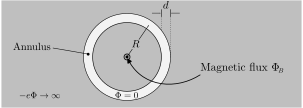
\includegraphics[width=0.4\textwidth]{annulus}
\end{figure}

Now, suppose we thread magnetic flux (e.g., using a solenoid) through
the origin, which lies in the region enclosed by the annulus.  This
flux can be described via the vector potential
\begin{equation}
  \mathbf{A}(r,\phi) = \frac{\Phi_B}{2\pi r} \, \hat{e}_\phi.
  \label{Asolenoid}
\end{equation}
We can verify from Eq.~\eqref{Asolenoid} that the magnetic flux
through any loop of radius $r$ enclosing the origin is $(\Phi_B/2\pi
r)(2\pi r) = \Phi_B$, independent of $r$.  Hence, the magnetic flux is
confined to an infintesimal area surrounding the origin, with
$\mathbf{B} = 0$ everywhere else. The vector potential $\mathbf{A}$,
however, is nonzero everywhere.

The time-independent Schr\"odinger equation is
\begin{equation}
  \frac{1}{2m}\left|-i\hbar\nabla+
  \frac{e\Phi_B}{2\pi r} \, \hat{e}_\phi\right|^2 \psi(r,\phi)
  = E\psi(r,\phi),
  \label{ABschrod}
\end{equation}
with the boundary conditions $\psi(R\pm d/2,0) = 0$.  For sufficiently
large $R$, we can guess that the eigenfunctions have the form
\begin{equation}
  \psi(r,\phi) \approx
  \psi_0 \, \cos\left(\frac{\pi}{d}(r-R)\right)\, e^{i k R \phi},
\end{equation}
where $\psi_0$ is a normalization constant.  This describes a waveform
with a half-wavelength wave profile in the $r$ direction (so as to
vanish at $r = R \pm d/2$), and traveling along the azimuthal
direction with wavenumber $k$.  In order for the wavefunction to be
single-valued,
\begin{equation}
  k \cdot 2\pi R = 2\pi n \;\;\;\Rightarrow \;\;\; k = \frac{n}{R},
  \;\;\;\mathrm{where}\;\; n \in \mathbb{Z}.
\end{equation}
Plugging this into Eq.~\eqref{ABschrod} yields the energy levels
\begin{align}
  E_n &= \frac{1}{2m} \left[
    \left(\frac{n\hbar}{R} + \frac{e\Phi_B}{2\pi R}\right)^2
    + \left(\frac{\pi\hbar}{d}\right)^2 \right] \\
  &= \frac{e^2}{8\pi^2mR^2} \left(\Phi_B + \frac{nh}{e} \right)^2
  + \frac{\pi^2\hbar^2}{2md^2}.
  \label{abcurves}
\end{align}
In the figure below, these energy levels are sketched versus the
magnetic flux $\Phi_B$.  According to Eq.~\eqref{abcurves}, the
energies are described by a set of quadratic curves, translated along
the $\Phi_B$ axis by integer multiples of $h/e$.  Evidently, varying
$\Phi_B$ will shift the eigen-energies in the annulus, despite the
fact that the magnetic field vanishes in the annulus.  This is a
manifestation of the Aharanov-Bohm effect.

\begin{figure}[h]
  \centering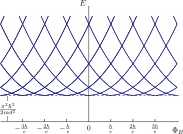
\includegraphics[width=0.65\textwidth]{abring}
\end{figure}

One very interesting feature of this energy spectrum is that it
remains the same whenever the magnetic flux changes by an exact
multiple of $h/e = 4.13567\times10^{-5}\,\mathrm{T}\,\mathrm{m}^2$.
This fundamental unit of magnetic flux is called the \textbf{magnetic
  flux quantum}.  Notably, it does not depend on the radius of the
annulus, or any other geometrical parameters of the system.  This is
because the invariance property arises from the gauge symmetry of the
Hamiltonian.  When an extra flux of $nh/e$ (where $n\in\mathbb{Z}$) is
threaded through the annulus, Eq.~\eqref{Asolenoid} tells us that the
change in vector potential is $\Delta \mathbf{A} = (n\hbar/ e r)
\hat{e}_\phi$.  We can undo the effects of this additional vector
potential using the gauge field
\begin{equation}
  \lambda(r,\phi) = \frac{n\hbar}{e} \, \phi \;\;\;\Rightarrow
  \begin{cases}\nabla \lambda &= \displaystyle (n\hbar/er) \hat{e}_\phi
    \\ \displaystyle e^{ie\lambda/\hbar} &= \displaystyle e^{in\phi}.
  \end{cases}
\end{equation}
Note that this gauge field is not single-valued, but it's not a
problem since both $\nabla\lambda$ and the phase factor
$\exp(ie\lambda/\hbar)$ remain single-valued.

\subsection{Non-relativistic electrons: the Pauli Hamiltonian}


\subsection{Relativistic electrons: the Dirac Hamiltonian}


\section{Quantizing the electromagnetic field}

\subsection{The electromagnetic field Hamiltonian}

\subsection{Relativity and quantum mechanics}

\section{The electron-photon interaction}

\subsection{The electromagnetic shift of energy levels}

Bethe's Lamb shift calculation.

\subsection{Photon emission and absorption}

Dirac's calculation of the coefficient of spontaneous emission.

\section{Looking ahead}

Need to treat both electrons and photons on the same footing, with QFT
language.  Renormalization.

\section*{Exercises}

\begin{enumerate}
\item Gauge transformations.
\end{enumerate}

\section*{Further Reading}

\begin{enumerate}[[1{]}]
\item A.~Zee, \textit{Quantum Field Theory in a Nutshell} (Princeton
  University Press, 2010).
\label{cite:zee}
\end{enumerate}

\end{document}


%% For decades after the discovery of quantum mechanics, the quantum
%% double-slit experiment was just a ``thought experiment'', meant to
%% illustrate the features of quantum mechanics that had been uncovered
%% by other, more complicated experiments.  Nowadays, the most convenient
%% way to do the experiment is with light, using single-photon sources
%% and single-photon detectors.  Quantum interference has also been
%% demonstrated experimentally using electrons, neutrons, and even
%% large-scale particles such as buckyballs.
